\subsection{dioganalsation} \label{chap_bench}

The performance of the MPO construction can be compared with the exact diagonalisation of the hamiltonian for a given number of sites. To obtain a faithful results, the number of sites should be as high as possible. In practice, diagonalisation of large matrices becomes slow and memory consuming. The size grows exponentially in the number of sites: $d^{n} \times d^{n} $. A double takes 8 bytes of memory.A Rough estimated of the amount of RAM $R$ needed to store this complex array is:

\begin{equation}
    R = d^{2 n} \times 16 bytes
\end{equation}

Which means a 14 site chain already takes up  GB of RAM.

\todo{time complexity algoritms}

\subsubsection{norms} \label{mponormdef}

\todo{trace norm, schatten p norm, ...}

The schatten 2 norm is used in the following analysis, dentoted by ${\| \cdot \|} _{2}$. In the figures the relative error $\epsilon$ is reported.

\def \expHBlock {\expH{4}{ $e^{- \beta \hat{H}_{n}}$   }{ {,,"...",} }{ {,,"...",} }{}{} }
\def \Mn {\mpo{4}{ {0,,,,0}  }{}{}{{0,0,1,0,0}}{}}

\begin{equation}
    \epsilon = \frac{  {  \left \|  \expHBlock - \Mn  \right \|} _{2}  }{ {  \left\|  \expHBlock \right \|}_2}
\end{equation}
\todo{make version for cyclic }

\paragraph{system size and cyclicity}

This norm can only be calculated for a finite number of sites. The influence of the number of sites for a linear  and cyclic \cref{benchmarking:systemsize} . As expected, the cyclic norm represents large systems better for the same number of sites. The linear norm keeps increasing with every added site.

Calculating the cyclic norm comes at the extra cost of contracting a cyclic tensor network. \todo{calculate complexity}

In this chapter, the cyclic norm will be given for M=8 sites.

\begin{figure}[H]
    \begin{subfigure}[]{\textwidth}
        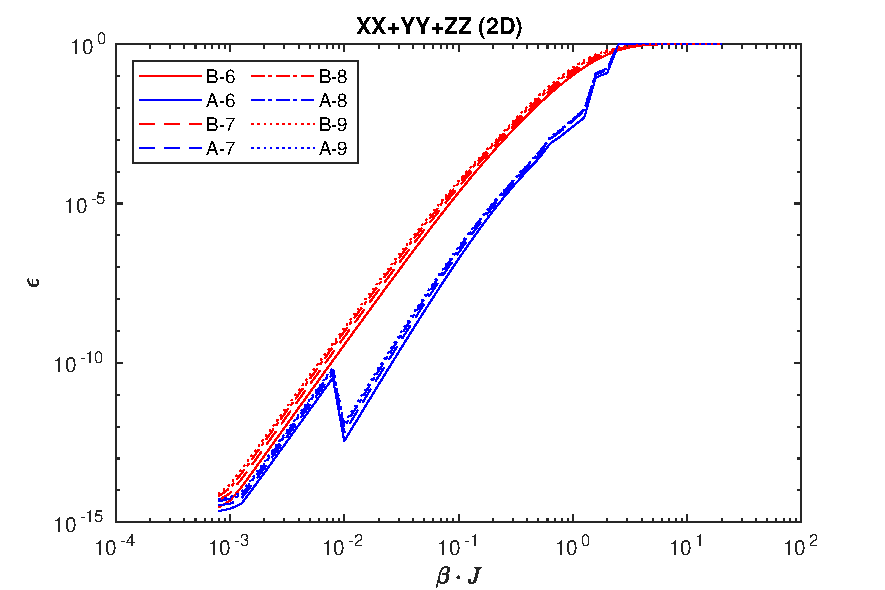
\includegraphics[width=\textwidth]{Figuren/benchmarking/keuze_norm/linear.pdf}
        \subcaption{test}
    \end{subfigure}

    \begin{subfigure}[]{\textwidth}
        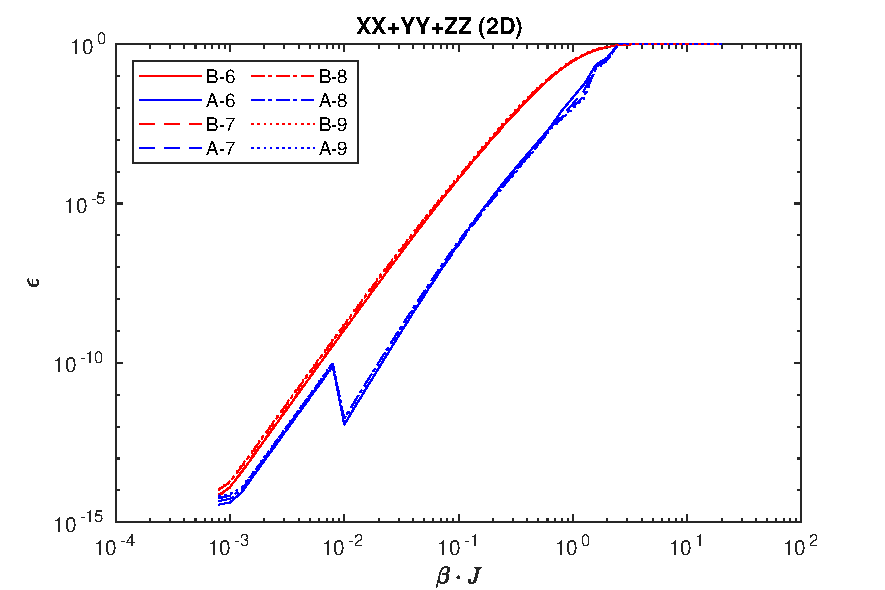
\includegraphics[width=\textwidth]{Figuren/benchmarking/keuze_norm/cyclic.pdf}
        \subcaption{test}
    \end{subfigure}
    \caption{test }
    \label{benchmarking:systemsize}
\end{figure}

\subsection{analytical results}